\section{Quantum dots}
    Artificial atoms, or the so-called quantum dots, constitute a hot topic in
    condensed matter physics and material sciences. We will be exploring
    several types of quantum dots in both one and two dimensions in this
    thesis. The difference between the types of quantum dots is found in the
    one-body potential. All of the dots share the characteristic of being in an
    infinite well which makes the systems \emph{bound}. In our study of systems
    subject to intense laser fields, this will prove to be a bad approximation
    when the laser becomes very strong as the particles have no way of being
    ionized, i.e., escape the potential well.  Even so, for weak laser fields
    and for ground state calculations, they serve as excellent candidates for
    our methods.

    \subsection{One-dimensional harmonic oscillator}
        One of the simplest theoretical models studied. The one-dimensional
        harmonic oscillator is usually one of the first models studied in
        undergraduate quantum mechanics courses. The one-body Hamiltonian of the
        one-dimensional harmonic oscillator is given by
        \begin{align}
            \onehamil = \frac{\momentum^2}{2m} + \half m\omega^2 \position^2,
            \label{eq:1dho-hamiltonian}
        \end{align}
        where the latter term, i.e., the one-body potential, gives rise to the
        name of the system. Plugging this operator into the time-independent
        Schrödinger equation
        \begin{gather}
            \onehamil\ket{n} = \epsilon_n\ket{n},
        \end{gather}
        which results in an energy eigenvalue equation we wish to solve in order
        to find an expression for $\ket{n}$.
        % TODO: Discuss both the algebraic derivation and the solution using
        % diagonalization on a grid.
        % TODO: Include analytic solution to \ket{n}.
        % TODO: Include figues of the potential and the eigenstates.

    \subsection{One-dimensional double well quantum dot}
        A slightly more complicated model is the \emph{double well} quantum dot.
        Succintly named due to its ``bump'' in the bottom of the parabolic
        potential from the harmonic oscillator. The one-body hamiltonian is
        given by
        \begin{align}
            \onehamil = \frac{\momentum^2}{2m}
            + \half m\omega^2\para{
                \position^2
                + \frac{1}{4}l^2
                - l\abs{\position}
            },
        \end{align}
        where $l$ is the ``width'' of the potential barrier in the bottom of the
        parabola.
        % TODO: What is the width? RMS?

    \subsection{Two-dimensional harmonic oscillator}
        The one-body Hamiltonian of the two-dimensional harmonic oscillator is
        virtually identical to the one-body Hamiltonian of the one-dimensional
        harmonic oscillator, i.e., \autoref{eq:1dho-hamiltonian}, but with the
        position and momentum operators being represented in two-dimensions. We
        will be looking at a circular, symmetric potential. We will thus be
        working in a polar coordinate basis. The main reason we choose
        the polar coordinate representation is due to the evaluation of the
        two-body Coulomb integral elements. This is the most costly part of the
        construction of the matrix elements and in a polar basis we have
        \emph{analytical} expressions for these elements
        \cite{anisimovas1998energy}.  The Hamiltonian can thus be represented by
        \begin{align}
            \onehamil &=
            \frac{\momentum^2}{2m}
            + \half m\omega^2\position[r]^2
            = -\frac{\hslash^2}{2m}\brak{
                \dpd[2]{}{r}
                + \frac{1}{r}\dpd[]{}{r}
                + \frac{1}{r^2}\dpd[2]{}{\theta}
            }
            + \half m \omega^2 \position[r]^2,
        \end{align}
        where $\position[r]^2 = \position^2 + \position[y]^2$. Next we insert
        the Hamiltonian into the time-independent Schrödinger equation
        \begin{align}
            \onehamil\ket{nm} = \epsilon_{nm}\ket{nm},
        \end{align}
        and diagonalize in order to find the eigenstates, $\ket{nm}$.
        Representing the eigenstates in polar coordinates
        \begin{align}
            \phi_{nm}(\vf{r}) = \phi_{nm}(r, \theta)
            \equiv \braket{r\theta}{nm},
        \end{align}
        we solve the eigenvalue problem by separating the radial and the angular
        part of the eigenstate and solve each term individually. That is,
        \begin{align}
            \phi_{nm}(r, \theta) = N_{nm}R_{nm}(r)\Theta_{m}(\theta).
            \label{eq:spf-2dqd}
        \end{align}
        % TODO: Complete this derivation, i.e., solve the differential equation and
        % find the normalization constant.
        % TODO: Talk about angular momentum.
        Solving the two coupled ordinary differential equations and finding the
        normalization constant, we find the terms
        \begin{align}
            N_{nm} = a\sqrt{\frac{n!}{\pi(n + \abs{m})!}},
        \end{align}
        as the normalization factor with
        \begin{align}
            a = \sqrt{\frac{m\omega}{\hslash}},
        \end{align}
        the Bohr radius. The radial contribution is given by
        \begin{align}
            R_{nm}(r)
            &= (ar)^{\abs{m}}L^{\abs{m}}_{n}(a^2r^2)
            \exp\brac{-\frac{a^2 r^2}{2}},
        \end{align}
        where $L^{m}_{n}(r)$ is the \emph{associated Laguerre polynomials}. The
        angular part is given by
        \begin{align}
            \Theta_m(\theta) = \exp\brac{im\theta}.
        \end{align}
        The eigenenergy, $\epsilon_{nm}$, of the two-dimensional eigenstates is
        given by
        \begin{align}
            \epsilon_{nm} = \hslash\omega\brak{
                2n + \abs{m} + 1
            }.
            \label{eq:eigenenergies_2dqd}
        \end{align}
        Staring at the eigenenergy equation we notice quite fast that the states
        are degenerate in the energy. A drawing of the first three energy levels
        with their corresponding quantum numbers is shown in
        \autoref{fig:2dho-energy-levels}.
        \begin{figure}
            \begin{center}
                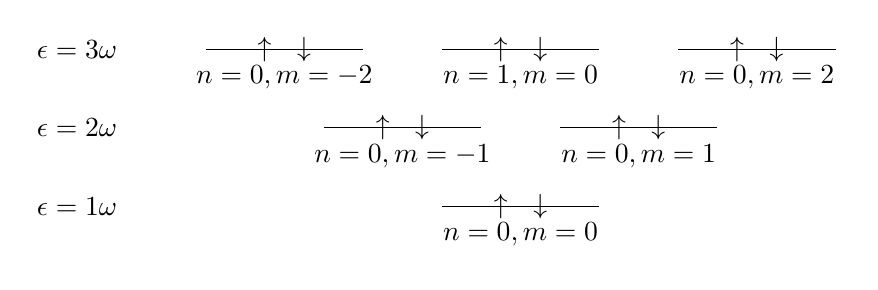
\begin{tikzpicture}
                    \begin{scope}
                        \foreach \i in {1, 2, 3} {
                            \draw(-1, \i - 1) node[anchor=east]
                            {$\epsilon = \i\hslash\omega$};
                        }

                        % Highest energy level
                        \foreach \i in {0, 3, 6} {
                            \draw (\i, 2) -- (\i + 2, 2);
                            \node at (\i + 0.75, 2) {$\uparrow$};
                            \node at (\i + 1.25, 2) {$\downarrow$};
                        }
                        \node[below, inner sep=.2cm] at (1, 2)
                        {$n = 0, m = -2$};
                        \node[below, inner sep=.2cm] at (4, 2)
                        {$n = 1, m = 0$};
                        \node[below, inner sep=.2cm] at (7, 2)
                        {$n = 0, m = 2$};

                        % Middle energy level
                        \foreach \i in {1.5, 4.5} {
                            \draw (\i, 1) -- (\i + 2, 1);
                            \node at (\i + 0.75, 1) {$\uparrow$};
                            \node at (\i + 1.25, 1) {$\downarrow$};
                        }
                        \node[below, inner sep=.2cm] at (2.5, 1)
                        {$n = 0, m = -1$};
                        \node[below, inner sep=.2cm] at (5.5, 1)
                        {$n = 0, m = 1$};

                        % Lowest energy level
                        \draw (3, 0) -- (5, 0);
                        \node at (3 + 0.75, 0) {$\uparrow$};
                        \node at (3 + 1.25, 0) {$\downarrow$};
                        \node[below, inner sep=.2cm] at (4, 0)
                        {$n = 0, m = 0$};
                    \end{scope}
                \end{tikzpicture}
            \end{center}
            \caption{In this plot we can see the energy degeneracy of the lowest
            three energy levels in the two-dimensional quantum dot.  Each arrow
            representes a spin up or a spin down state with the quantum numbers
            $n$ and $m$ as listed below. This pattern goes on indefinitly with
            the addition of one bar (two oscillators) per level.}
            \label{fig:2dho-energy-levels}
        \end{figure}
        The basis functions are orthonormal. By including spin as a quantum
        number $\sigma$, we can represent this by
        \begin{align}
            \braket{n_1 m_1 \sigma_1}{n_2 m_2 \sigma_2}
            = \delta_{n_1 n_2}\delta_{m_1 m_2} \delta_{\sigma_1 \sigma_2}.
        \end{align}
        % TODO: Add "mexican-hat" plots of probability density

        \subsubsection{Mapping the quantum numbers to a single value}
            When working with second quantized operators, we distinguish single
            particle functions in a Slater determinant by a single index.
            Including spin in the two-dimensional harmonic oscillator
            eigenstates we have to deal with three quantum numbers $n$, $m$ and
            $\sigma$ per state.  We are thus interested in finding a mapping
            $(n, m) \mapsto p$ and the inverse mapping $p \mapsto (n,
            m)$\footnote{The spin quantum number is easiest to deal with in the
            end as we can double each dimension in every tensor and label all
            odd or even indices by a spin direction.}.  Due to the degeneracy of
            the eigenenergies such a mapping will not be unique. We thus have to
            decide in advance how we should count the basis states. In this
            thesis we choose the convention that we start from the lowest energy
            level and move up by counting from left to right. Tabulating
            \autoref{fig:2dho-energy-levels} we get the table shown in
            \autoref{tab:2dho-mapping}.  In \autoref{alg:nm-to-p} we give a
            sketch of the algorithm we use to compute $(n, m) \mapsto p$. We
            show the inverse algorithm in \autoref{alg:p-to-nm}.

            Using the aforementioned mapping we can find indices $p$ such that
            \begin{align}
                \ket{nm} \mapsto \ket{p}.
            \end{align}

            \begin{table}
                \centering
                \caption{In this table we show an example of how our mapping
                convention will index the states shown in
                \autoref{fig:2dho-energy-levels}.}
                \begin{tabular}{c|ll}
                    $\epsilon_{nm}$ & $(n, m)$ & $p$ \\
                    \hline
                    \\
                    \hslash\omega & $(0, 0)$ & $0$ \\
                    2\hslash\omega & $(0, -1)$ & $1$ \\
                    2\hslash\omega & $(0, 1)$ & $2$ \\
                    3\hslash\omega & $(0, -2)$ & $3$ \\
                    3\hslash\omega & $(1, 0)$ & $4$ \\
                    3\hslash\omega & $(0, 2)$ & $5$
                \end{tabular}
                \label{tab:2dho-mapping}
            \end{table}

            \begin{algorithm}
                \caption{In this algorithm we describe how we can find $(n, m)
                \mapsto p$ relatively quick without having to tabulate all
                maps.}
                \label{alg:nm-to-p}
                \begin{algorithmic}[1]
                    \Function{map-nm-to-p}{$n, m$}
                    \State $s \gets 2n + \abs{m} + 1$
                    \Comment{Compute shell number $s$}
                    \State $n_0 \gets \sum_{i = 1}^{s - 1} i$
                    \Comment{Count the number of states up to shell $s$}
                    \State $n_f \gets n_0 + s$
                    \Comment{Count the number of states including $s$}
                    \If{$m = 0$}
                        \If{$n = 0$}
                            \State \textbf{return} $0$
                            \Comment{Lowest state, i.e., $p = 0$}
                        \EndIf
                        \State $p = n_0 + (n_f - n_0)/2$
                        \Comment{We must be in the middle of a shell where $s =
                        2n + 1$}
                        \State \textbf{return} $p$
                    \ElsIf{$m < 0$}
                        \State $p = n_0 + n$
                        \Comment{Count the number of states from previous shell}
                        \State \textbf{return} $p$
                    \Else
                        \State $p = n_f - (n + 1)$
                        \Comment{Count the number of states from top of current
                        shell}
                        \State \textbf{return} $p$
                    \EndIf
                    \EndFunction
                \end{algorithmic}
            \end{algorithm}

            \begin{algorithm}
                \caption{In this algorithm we sketch how we can find $p \mapsto
                (n, m)$, i.e., the inverse of \autoref{alg:nm-to-p}.}
                \label{alg:p-to-nm}
                \begin{algorithmic}[1]
                    \Function{map-p-to-nm}{$p$}
                    \State $n_p \gets 0$
                    \Comment{Initialize variable to keep track of previous
                    shell}
                    \State $n_c \gets 1$
                    \Comment{Initialize variable to keep track of current shell}
                    \State $s_c \gets 1$
                    \Comment{Initialize the shell counter. This serves as a
                    cumulative sum for $n_c$}
                    \While{$n_c \leq p$}
                        \Comment{Check if $p$ is included in the current shell}
                        \State $s_c \gets s_c + 1$
                        \Comment{Increase shell counter}
                        \State $n_p \gets n_c$
                        \Comment{Store number of particles in previous shell}
                        \State $n_c \gets n_p + s_c$
                        \Comment{Add number of particles to current shell}
                    \EndWhile
                    \State $p_c = (n_c - n_p) / 2 + n_p$
                    \Comment{Compute the index $p$ of the middle of a shell}
                    \If{$n_c - n_p = 2k + 1$}
                        \Comment{Check if current shell has an odd number of
                        particles}
                        \If{$p = p_c$}
                            \Comment{Check if $p$ is in the middle}
                            \State $n \gets s_c / 2$
                            \Comment{The shell is computed from $s_c = 2n + 1$}
                            \State $m \gets 0$
                            \State \textbf{return} $(n, m)$
                        \EndIf
                    \EndIf
                    \If{$p < p_c$}
                        \Comment{Check if we have negative $m$}
                        \State $n \gets p - n_p$
                        \Comment{Count up from previous shell}
                        \State $m \gets -((s_c - 1) - 2n)$
                        \State \textbf{return} $(n, m)$
                    \Else
                        \Comment{We have positive $m$}
                        \State $n \gets (n_c - 1) - p$
                        \Comment{Count down from current shell}
                        \State $m \gets (s_c - 1) - 2n$
                        \State \textbf{return} $(n, m)$
                    \EndIf
                    \EndFunction
                \end{algorithmic}
            \end{algorithm}

        \subsubsection{Computing the dipole moments}
            The matrix elements of the dipole moment of the two-dimensional
            harmonic oscillator quantum dot is given by
            \begin{align}
                \vf{d}_{ij}
                \equiv \bra{i}\position[\vf{r}]\ket{j},
            \end{align}
            where we get a dipole moment for each coordinate in $\vf{r}$. As
            we've expressed the single particle functions in polar coordinates,
            but wish to express the dipole moments in a cartesian coordinate
            system, we have to compute the two integrals
            \begin{align}
                \vf{d}_{ij}
                &= \vf{i}\bra{i} \position\ket{j}
                + \vf{j}\bra{i} \position[y]\ket{j}
                = \vf{i}\bra{i} r \cos(\theta)\ket{j}
                + \vf{j}\bra{i} r \sin(\theta)\ket{j},
                \label{eq:dipole_elements}
            \end{align}
            where $\vf{i}$ and $\vf{j}$ are the unit vectors along the $x$- and
            $y$-axis respectively.  Using \autoref{eq:spf-2dqd} we are able to
            find analytical expressions for the angular integral. The radial
            integral must be evaluated from $0$ to $\infty$, but lucikly SymPy
            \cite{sympy} handles this for us. Note that we use the notation $i
            \mapsto (n_i, m_i)$ from the mapping algorithms described above. We
            then get the following integrals
            \begin{align}
                \bra{i} r \cos(\theta) \ket{j}
                &= N^{*}_{n_i m_i} N_{n_j m_j}
                \int_{0}^{\infty} \dd r r^2
                R_{n_i m_i}^{*}(r) R_{n_j m_j}(r)
                \int_{0}^{2\pi} \dd \theta \cos(\theta)
                \Theta_{m_i}^{*}(\theta) \Theta_{m_j}(\theta)
                \\
                &= N^{*}_{n_i m_i} N_{n_j m_j} I_{r} I_{\theta_1},
                \\
                \bra{i} r \sin(\theta) \ket{j}
                &= N^{*}_{n_i m_i} N_{n_j m_j}
                \int_{0}^{\infty} \dd r r^2
                R_{n_i m_i}^{*}(r) R_{n_j m_j}(r)
                \int_{0}^{2\pi} \dd \theta \sin(\theta)
                \Theta_{m_i}^{*}(\theta) \Theta_{m_j}(\theta)
                \\
                &= N^{*}_{n_i m_i} N_{n_j m_j} I_{r} I_{\theta_2}.
            \end{align}
            We use Wolfram Alpha to solve the $I_{\theta_1}$ and $I_{\theta_2}$
            integrals giving a closed form solution. For $I_{\theta_1}$ we get
            \cite{wolframalphai1}
            \begin{align}
                I_{\theta_1}
                &=
                \int_{0}^{2\pi} \dd \theta \cos(\theta)
                \Theta_{m_i}^{*}(\theta) \Theta_{m_j}(\theta)
                =
                \int_{0}^{2\pi} \dd \theta \cos(\theta)
                \exp\brac{i(m_j - m_i)\theta}
                \\
                &=
                - \frac{
                    i\brak{
                        -1 + \exp\brac{2i\pi(m_j - m_i)}
                    }\brak{m_j - m_i}
                }{
                    \brak{m_j - m_i}^2 - 1
                }.
            \end{align}
            Paying close attention to the case when $\abs{m_j - m_i} = 1$ as
            this seems to blow up. Luckily, this yields $I_{\theta_1} = \pi$
            \cite{wolframalphai1-zero}. For the $I_{\theta_2}$-integral we get
            \cite{wolframalphai2}
            \begin{align}
                I_{\theta_2}
                &=
                \int_{0}^{2\pi} \dd \theta \sin(\theta)
                \Theta_{m_i}^{*}(\theta) \Theta_{m_j}(\theta)
                =
                \int_{0}^{2\pi} \dd \theta \sin(\theta)
                \exp\brac{i(m_j - m_i)\theta}
                \\
                &=
                \frac{\exp\brac{2i\pi(m_j - m_i)} - 1}{\brak{m_j - m_i}^2 - 1},
            \end{align}
            where we again explicitly check that we get a finite result for
            $\abs{m_j - m_i} = 1$. This yields $I_{\theta_2} = i\pi$
            \cite{wolframalphai2-zero}.

        \subsubsection{Computing the Coulomb elements}
            Having found the basis functions and the elements of the one-body
            hamiltonian, we are left with the task of finding the two-body
            elements from the Coulomb interaction. Luckily, there exists an
            analytic formula finding these elements. This formula is shown in
            appendix A in the article \citetitle{anisimovas1998energy} by
            \citeauthor{anisimovas1998energy} \cite{anisimovas1998energy}. Note
            that \citeauthor{anisimovas1998energy} interchanges the indices in
            the ket-part of their two-body integrals as opposed to our
            convention. That is, in our notation we would write
            \begin{align}
                \bra{ij}\twohamil\ket{kl}
                &= \delta_{ik}\delta_{jl}
                \int\dd x_1\dd x_2
                \phi_{i}^{*}(x_1) \phi_{j}^{*}(x_2)
                \twohamil
                \phi_{k}(x_1)\phi_{l}(x_2)
                \equiv
                \bra{ij}\twohamil\ket{lk}_{AM},
            \end{align}
            where $ \bra{ij}\twohamil\ket{lk}_{AM}$ is the convention used by
            \citeauthor{anisimovas1998energy}.
            % TODO: Consider writing the full formula.
            % This can be added in the appendix.
            % Add comment on implementation, and who gave it to you.


    \subsection{Two-dimensional double well quantum dot}
        A more interesting system to peruse is the double well quantum dot.
        We'll specifically be looking at the two-dimensional double well quantum
        dot as this lets us reuse the machinery from the two-dimensional
        harmonic oscillator quantum dot.
        There are a multitude of ways to create a confining double well
        potential.
        In the following we'll be focusing on a double well with a sharp
        boundary for the barrier in either $x$- or $y$-direction.
        The one-body Hamiltonian of the double well with the barrier in the
        $x$-direction is given by
        \begin{align}
            \onehamil
            &=
            \frac{\momentum^2}{2m}
            + \half m \omega^2 \position[r]^2
            + \half m \omega^2 \para{
                \frac{1}{4} l^2 - l\abs{\position}
            }.
            \label{eq:one-body-2ddw}
        \end{align}
        % TODO: Give motivation for the shape of the double-well.
        In \autoref{eq:one-body-2ddw} we recognize the two first terms as the
        kinetic energy and the harmonic oscillator confining potential.
        Instead of finding an analytical expression for the full one-body
        Hamiltonian\footnote{%
            An analytical expression might not even exist.
        }, as we did for the harmonic oscillator, we'll instead re-use
        the single-particle functions in \autoref{eq:spf-2dqd}.
        The one-body matrix elements can then be found from
        \begin{align}
            \oneten^{p}_{q}
            &= \epsilon_{p}\delta^{p}_{q}
            + \half m \omega^2\bra{p}\para{
                \frac{1}{4} l^2 - l \abs{\position}
            }\ket{q}
            \\
            &= \epsilon_{p}\delta^{p}_{q}
            + \frac{1}{8} m \omega^2 l^2 \delta^{p}_{q}
            - \half m \omega^2 l \bra{p}\abs{\position}\ket{q},
        \end{align}
        where we have used the mapping $(n, m) \to p$ described above and where
        the eigenenergies $\epsilon_p$ are given by
        \autoref{eq:eigenenergies_2dqd}.
        The two first terms give a shifted harmonic oscillator potential, viz.
        \begin{align}
            \epsilon_p' = \epsilon_p + \frac{1}{8} m \omega^2 l^2.
        \end{align}
        The last term is the double well barrier and resembles the dipole matrix
        elements from \autoref{eq:dipole_elements} except for the absolute
        value.
        As we've expressed the harmonic oscillator eigenfunctions in a radial
        basis, we'll compute the integrals in a radial coordinate system.
        \begin{align}
            \bra{p}\abs{\position}\ket{q}
            &=
            \int_{0}^{\infty}\int_{0}^{2\pi}
            \dd r \dd\theta
            \phi_{n_p m_p}^{*}(r, \theta)
            r^2\abs{\cos(\theta)}
            \phi_{n_q m_q}(r, \theta).
        \end{align}
        If we were to have a barrier in the $y$-direction we would replace the
        cosine with a sine. Using \autoref{eq:spf-2dqd} for the basis functions,
        we see that the normalization factor and the radial integral is the same
        as for the dipole moment of the two-dimensional harmonic oscillator
        quantum dot. The only difference is the absolute value on the periodic
        function in the polar integral. This gives \cite{wolframalphatildei1}
        \begin{align}
            \tilde{I}_{\theta_1}
            &=
            \int_{0}^{2\pi}\dd \theta \abs{\cos(\theta)}
            \Theta_{m_p}^{*}(\theta)
            \Theta_{m_q}(\theta)
            =
            \int_{0}^{2\pi}\dd \theta \abs{\cos(\theta)}
            \exp\brac{i(m_q - m_p)\theta}
            \\
            &=
            -i\brak{
                p + q
                + (p - q)\exp\brac{i\pi(p - q)}
                - 2i\exp\brac{
                    i\pi(p - q)/2
                }
            }
            \\
            &\qquad
            \times
            \frac{
                % This term should be 1:
                % \exp\brac{-2i\pi(m_p - m_q)}
                \brak{
                    1 + \exp\brac{i\pi(m_p - m_q)}
                }
            }{
                \para{m_q - m_p}^2 - 1
            },
        \end{align}
        where we've labeled the integral in the $x$-direction
        $\tilde{I}_{\theta_1}$.
        When $\abs{m_q - m_p} = 1$ we get $\tilde{I}_{\theta_1} = 0$
        \cite{wolframalphatildei1-zero}.
        For the $y$-direction we get the integral \cite{wolframalphatildei2}
        \begin{align}
            \tilde{I}_{\theta_2}
            &=
            \int_{0}^{2\pi}\dd \theta \abs{\sin(\theta)}
            \Theta_{m_p}^{*}(\theta)
            \Theta_{m_q}(\theta)
            =
            \int_{0}^{2\pi}\dd \theta \abs{\sin(\theta)}
            \exp\brac{i(m_q - m_p)\theta}
            \\
            &=
            -\frac{
                \brak{
                    1 + \exp\brac{i \pi (m_q - m_p)}
                }^2
            }{
                \para{m_q - m_p}^2 - 1
            }.
        \end{align}
        When $\abs{m_q - m_p} = 1$ this integral yields $\tilde{I}_{\theta_2} =
        0$ \cite{wolframalphatildei2-zero}.
